\documentclass[../notes.tex]{subfiles}

\pagestyle{main}
\renewcommand{\chaptermark}[1]{\markboth{\chaptername\ \thechapter\ (#1)}{}}
\stepcounter{chapter}

\begin{document}




\chapter{\emph{N}-Doped Heterocycles}
\section{Benzannulated Pyridine Derivatives}
\begin{itemize}
    \item \marginnote{1/11:}Announcements.
    \begin{itemize}
        \item Next week: Thursday lecture only.
        \item Reiterates that we should try the problems, but don't fret.
    \end{itemize}
    \item Today: An hour of lecture, and a half hour of problems.
    \item New heterocycles: \textbf{Quinoline} and \textbf{isoquinoline}.
    \begin{figure}[h!]
        \centering
        \footnotesize
        \begin{subfigure}[b]{0.2\linewidth}
            \centering
            \chemfig{*6(\charge{-150={\tiny\color{grx}$7$}}{}=\charge{-90={\tiny\color{grx}$8$}}{}(-[6,0.45,,,opacity=0])-*6(=\charge{[extra sep=4pt]-90={\tiny\color{grx}$1$}}{N}-\charge{-30={\tiny\color{grx}$2$}}{}=\charge{30={\tiny\color{grx}$3$}}{}-\charge{90={\tiny\color{grx}$4$}}{}=)--\charge{90={\tiny\color{grx}$5$}}{}=\charge{150={\tiny\color{grx}$6$}}{}-)}
            \caption{Quinoline.}
            \label{fig:quinolineDeriva}
        \end{subfigure}
        \begin{subfigure}[b]{0.2\linewidth}
            \centering
            \chemfig{*6(\charge{-150={\tiny\color{grx}$7$}}{}=\charge{-90={\tiny\color{grx}$8$}}{}(-[6,0.45,,,opacity=0])-*6(=\charge{[extra sep=4pt]-90={\tiny\color{grx}$1$}}{}-\charge{0={\tiny\color{grx}$2$}}{N}=\charge{30={\tiny\color{grx}$3$}}{}-\charge{90={\tiny\color{grx}$4$}}{}=)--\charge{90={\tiny\color{grx}$5$}}{}=\charge{150={\tiny\color{grx}$6$}}{}-)}
            \caption{Isoquinoline.}
            \label{fig:quinolineDerivb}
        \end{subfigure}
        \begin{subfigure}[b]{0.2\linewidth}
            \centering
            \chemfig{*6(\charge{-150={\tiny\color{grx}$7$}}{}=\charge{-90={\tiny\color{grx}$8$}}{}(-[6,0.45,,,opacity=0])-*6(=\chembelow{\charge{[extra sep=2.5pt]-160={\tiny\color{grx}$1$}}{N}}{H}-\charge{-30={\tiny\color{grx}$2$}}{}=\charge{30={\tiny\color{grx}$3$}}{}-\charge{[extra sep=4.5pt]155={\tiny\color{grx}$4$}}{}(=O)-)=-\charge{90={\tiny\color{grx}$5$}}{}=\charge{150={\tiny\color{grx}$6$}}{}-)}
            \caption{4-quinolone.}
            \label{fig:quinolineDerivc}
        \end{subfigure}
        \caption{Key quinoline derivatives.}
        \label{fig:quinolineDeriv}
    \end{figure}
    \vspace{-0.3em}
    \begin{itemize}
        \item Important subclass: Quinine- and \textbf{quinolone}-derived drugs.
        % \begin{itemize}
        %     \item Both 2- and 4-quinolones are important.
        % \end{itemize}
        \item Comparison with pyridine: Quinolines have two different aromatic regions.
    \end{itemize}
    \item We'll now discuss some basic quinoline reactivity patterns.
    \item Relative EAS reactivity.
    \begin{equation*}
        \text{Benzene}>\text{Isoquinolinium}>\text{Quinolinium}\gg\text{Pyridinium}
    \end{equation*}
    \vspace{-1.7em}
    \item Quinoline (dissolved in pyridine) can react to give the 3-bromoquinoline.
    \begin{figure}[H]
        \centering
        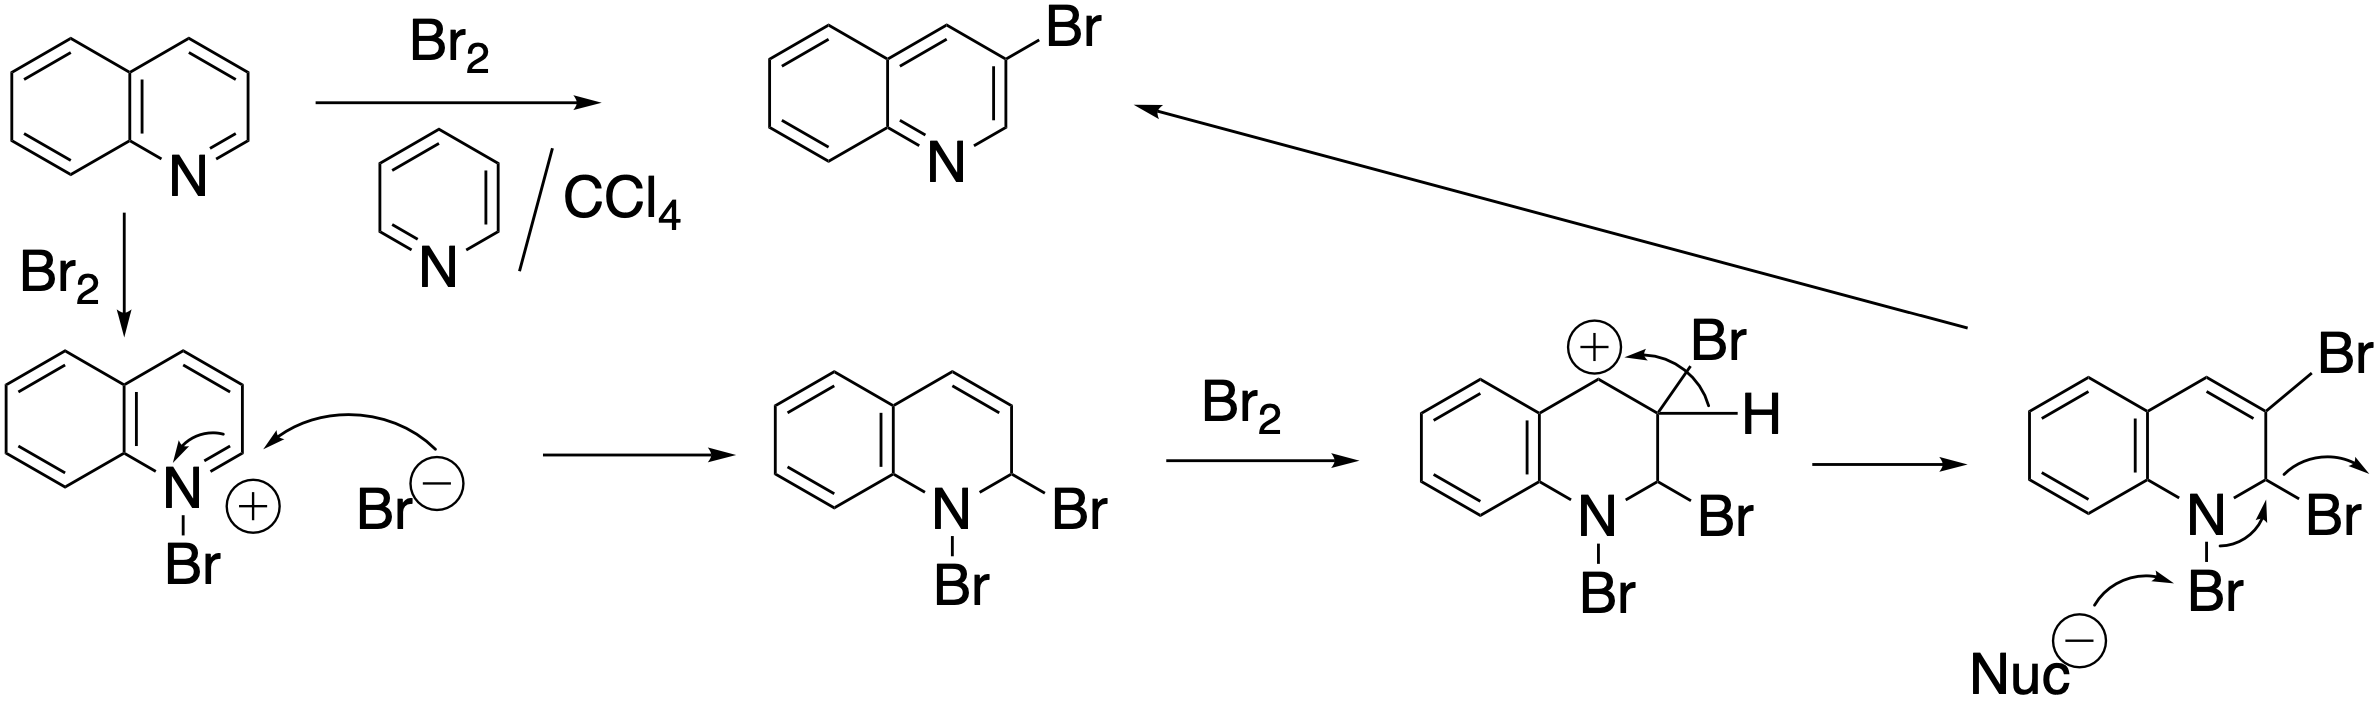
\includegraphics[width=0.8\linewidth]{QI3bromoMech.png}\\[-0.5em]
        \caption{Quinoline 3-bromination mechanism.}
        \label{fig:QI3bromoMech}
    \end{figure}
    \begin{itemize}
        \item However, the reaction mechanism is \emph{not} EAS.
        \item Indeed, this reaction is feasible only because a different mechanism is operational.
    \end{itemize}
    \item Lithiates --- followed by oxidation --- add to quinoline at the 2-position.
    \begin{figure}[h!]
        \centering
        \begin{subfigure}[b]{\linewidth}
            \centering
            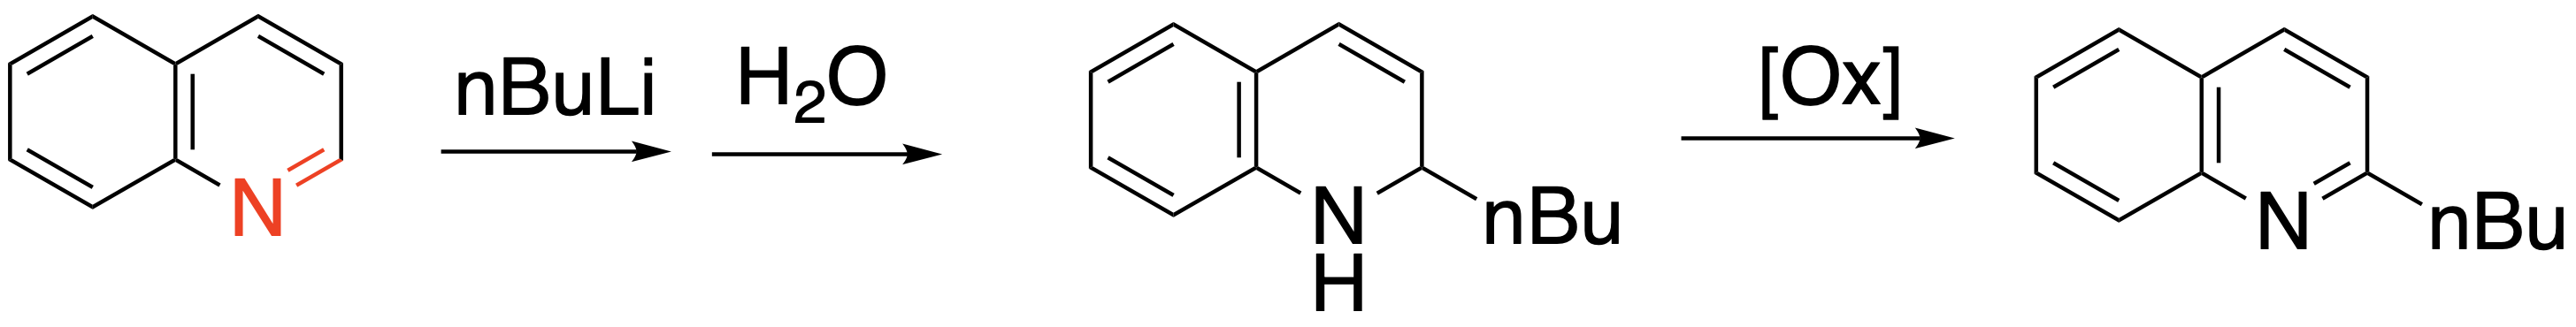
\includegraphics[width=0.63\linewidth]{QILia.png}
            \caption{Monoaddition.}
            \label{fig:QILia}
        \end{subfigure}\\[2em]
        \begin{subfigure}[b]{\linewidth}
            \centering
            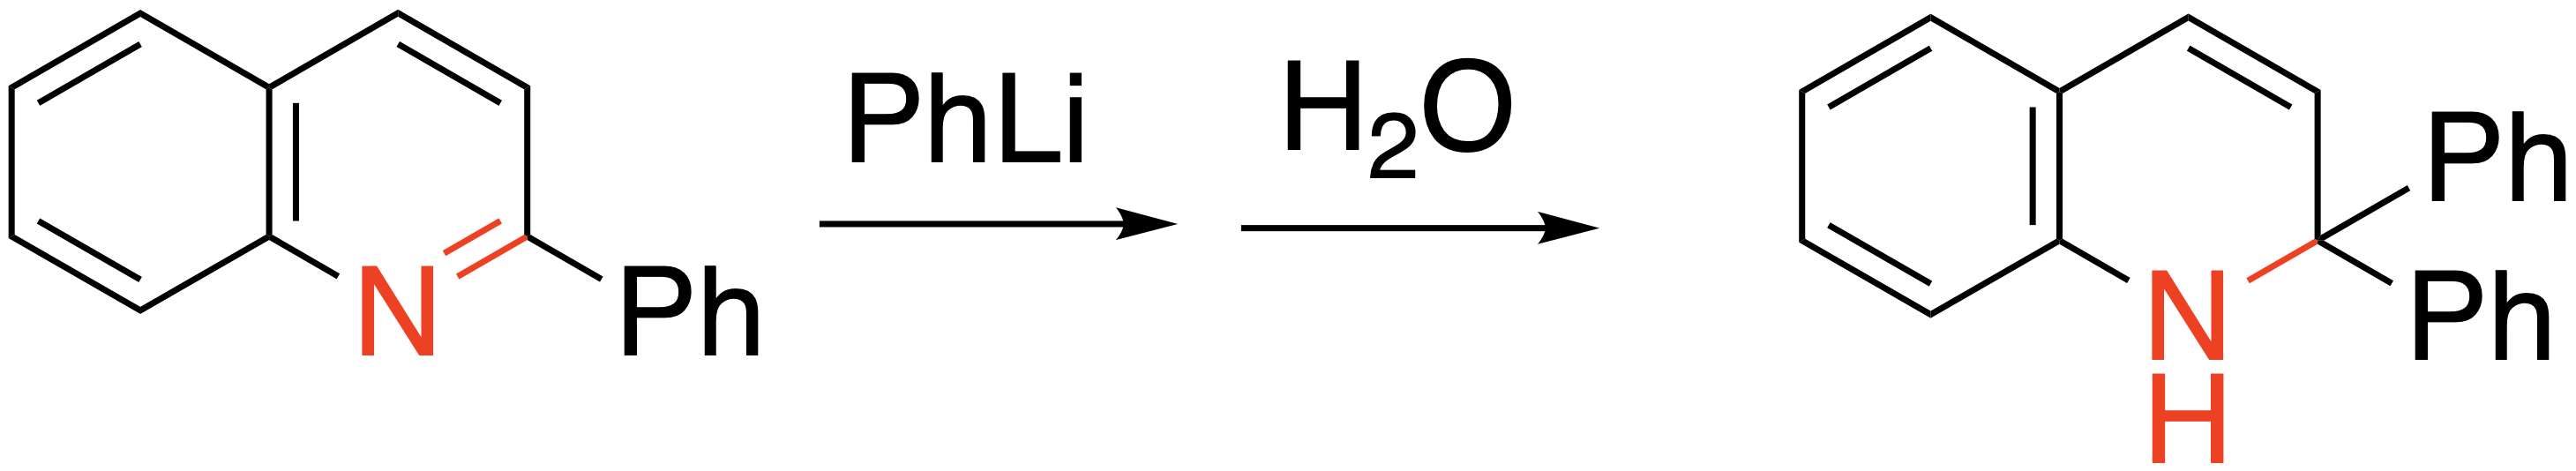
\includegraphics[width=0.41\linewidth]{QILib.png}
            \caption{Diaddition.}
            \label{fig:QILib}
        \end{subfigure}
        \caption{Lithiates add to quinoline.}
        \label{fig:QILi}
    \end{figure}
    \begin{itemize}
        \item We can also use analogous approaches to dearomatize the pyridine moiety by making a quaternary carbon.
        \item Lithium-nitrogen coordination is critical to 2-addition; otherwise, we get 4-addition.
    \end{itemize}
    \item Quinoline syntheses.
    \begin{itemize}
        \item Many different ones, many from Germany.
        \item Most common: \textbf{Skraup}, \textbf{Conrad-Limpach-Knorr}, and \textbf{Meth-Cohn} syntheses.
        \item For most of these, you start with the aniline.
        \item Common issues: Mixture of regioisomers.
    \end{itemize}
    \item Meth-Cohn quinoline synthesis.
    \begin{itemize}
        \item Proceeds via a mechanism analogous to the \textbf{Vilsmeier-Haack reaction}.
        \item Driving force: \ce{P=O} bond formation.
        \item Amide $\to$ chloroimine, tautomerizes to enamine. Then an additional carbon comes from DMF.
    \end{itemize}
    \item Quinoline hydrogenations.
    \begin{itemize}
        \item You can get some interesting chemoselectivity, enabling you to reach basically whatever you want!
        \item Reducing the benzene ring.
        \begin{itemize}
            \item Completely counterintuitive result: In the presence of an acid, you reduce the non-heterocyclic part of the quinoline heterocycle.
        \end{itemize}
        \item Reducing the heterocyclic ring, or everything: Use Raney nickel (RaNi).
        \begin{itemize}
            \item RaNi is a pyrophoric, extremely active form of nickel used for very difficult hydrogenations and desulfurizations.
            \item Under \SI{1}{\atmosphere} of \ce{H2}, you'll only hydrogenate the heterocyclic ring.
            \item Under \SI{70}{\atmosphere} of \ce{H2}, you'll hydrogenate everything (typically to the \emph{cis}-decalin derivative, but you can get some isomers).
        \end{itemize}
    \end{itemize}
    \item Most famous quinoline synthesis: The Skraup quinoline synthesis.
    \begin{itemize}
        \item Michael addition, Friedel-Crafts type cyclization, and oxidation.
        \item A series of conditions for this reaction have been optimized over time.
        \item Classic Skraup.
        \begin{itemize}
            \item Reagents: Glycerol, sulfuric acid, and \ce{As2O5} (oxidizing agent).
            \item Under acidic conditions, glycerol will lose 2 equivalents of \ce{H2O} to generate acrolein \emph{in situ}.
            \begin{itemize}
                \item Following protonation, the first step involves a hydride shift to $\beta$-hydroxyaldehyde.
                \item Then we get E\textsubscript{1} via the electron conduit to acrolein.
            \end{itemize}
            \item Why don't we just add acrolein directly?
            \begin{itemize}
                \item Glycerol is really safe and cheap, but acrolein will "polymerize if you look at it sideways."
                \item Substituted acrolein derivatives (e.g., other Michael acceptors) can be added directly with sulfuric or tosylic acid, but acrolein, itself, needs these conditions.
            \end{itemize}
            \item Using Skraup methodology, we can synthesize 1,10-phenanthroline from 8-aminoquinoline.
            \item But not super scalable: Reaction "often resulted in uncontrolled violence."
        \end{itemize}
        \item Scalable Skraup.
        \begin{itemize}
            \item Alternative: Use glycerol in the presence of iron sulfate, a strong acid (e.g., methane sulfonic acid), and a strong oxidant (deprotonated sulfonic acid).
            \begin{itemize}
                \item The use of this particular oxidant makes separation easier at the end.
                \item This is an unusual use of a nitro group as an oxidizing agent; not often used, but was recently by Baran.
            \end{itemize}
            \item Once acrolein is generated \emph{in situ}, it undergoes Michael addition. Then we get Friedel-Crafts reactivity, followed by oxidation.
            \item This method was used to synthesize a PDE4 inhibitor.
        \end{itemize}
    \end{itemize}
    \item Misc. quinoline derivative syntheses.
    \begin{itemize}
        \item \textbf{Combes} (quinoline synthesis): Aniline condenses with a $\beta$-diketone, followed by intramolecular acid-promoted Friedel-Crafts cyclization.
        \item \textbf{Conrad-Limpach-Knorr} (quinolone synthesis): The mechanism involves a Combes-analogous condensation with a $\beta$-ketoester, followed by Friedel-Crafts cyclization.
        \begin{itemize}
            \item Sulfuric acid gives the 2-quinolone product.
            \item Heat gives the 4-quinolone product.
            \item We'll discuss this difference later!
        \end{itemize}
        \item Used to make compounds that fight botulism, malaria, and ebola.
        \begin{itemize}
            \item One important reagent used in some syntheses is \textbf{Eaton's reagent}.
        \end{itemize}
    \end{itemize}
    \item \textbf{Eaton's reagent}: \ce{MeSO3H} + \ce{P2O5}.
    \begin{itemize}
        \item This is a variation on PPA from last time. Easier to work with an quantitate.
    \end{itemize}
    \item Making a KRAS inhibitor.
    \begin{itemize}
        \item KRAS is a particularly virulent form of cancer for which inhibitors have not come on the market until recently.
        \item The starting material is a trisubstituted anline that is probably not cheap.
        \item Selectively (or selectively enough) chlorinate this SM.
        \begin{itemize}
            \item On an exam, Steve will never ask us to think that we could do this selectively.
            \item It's not obvious to him that we would chlorinate where we do, but we \emph{should} be able to draw a mechanism!! (This is basically 5.12 chem.)
        \end{itemize}
        \item \textbf{Meldrum's acid} and a trimethyl orthoester condense into a new reagent.
        \begin{itemize}
            \item This reagent is very prone to nucleophilic attack, so we get a Michael-type addition-elimination condensation with the aniline.
        \end{itemize}
        \item Then heating the mixture to boiling using Dowtherm as a solvent causes the substrate to collapse to the quinolone.
        \begin{itemize}
            \item The mechanism for this is at the bottom in the box.
            \item Note that at high temperatures, Meldrum's acid is known to undergo a pericyclic decomposition to a ketene, \ce{CO2}, and acetone; evidently, only acetone gets kicked out here, not \ce{CO2}.\footnote{\href{https://en.wikipedia.org/wiki/Meldrum's_acid\#Synthesis_of_ketenes}{Wikipedia}. Note also that Meldrum's acid is so strong because the conformational restriction caused by the ring forces the $\alpha$-proton to undergo $\sigma_{\ce{CH}}\to\pi^*_{\ce{CO}}$ donation.}
            \item In fact, it appears that the whole mechanism in the box plausibly occurs via a sequence of pericyclic reactions.
        \end{itemize}
        \item Nitric acid then gives nitration.
        \item \ce{POCl3} chlorinates the ketone and aromatizes the system.
        \item Pretty selective S\textsubscript{N}Ar occurs, even with a hindered piperazine.
        \item A note of the mechanism of action: Acrylimides (top of the finished molecule) are thought to give Michael addition with DNA.
    \end{itemize}
    \item \textbf{Friedlander} (quinoline synthesis).
    \begin{itemize}
        \item Retrosynthetic disconnections: An alkene disconnects into a carbanion equivalent and a carbonyl, and an imine disconnects into an amine and a carbonyl.
        \begin{itemize}
            \item Very rational.
        \end{itemize}
        \item Subject to regiocontrol issues.
        \begin{itemize}
            \item McWilliams (at Pfizer) did a very careful study, and was able to use an organocatalyst to get 90\% selectivity for one regioisomer.
        \end{itemize}
        \item Aside: Scalability.
        \begin{itemize}
            \item 90\% selectivity may not sound great to us.
            \item But as long as we can reject the unwanted isomer via recrystallization or derivitization (not chromatography), this is much better than a 4-step synthesis that requires complicated/expensive reagents or conditions.
        \end{itemize}
        \item This chemistry is generalizable, as well; see the reaction at the bottom of the slide.
        \item Anytime the symbol "OEi" appears in a slide, that means "$\Delta$."
    \end{itemize}
    \item Example synthesis: A MS drug by UCB (a Belgian pharmaceutical company).
    \begin{itemize}
        \item Starting material: A nitro-phenylalanine derivative.
        \item Condensation to the amide with a variant of Yamaguchi's reagent.
        \item Reduction of the nitro group to the corresponding aniline.
        \item Condensation with a dichlorobenzaldehyde to form the imine.
        \item \textbf{Pavarov reaction} with a good leaving group.
        \begin{itemize}
            \item Specifically, 2-pyrrolidone leave under oxidative conditions.
        \end{itemize}
        \item Lastly, we hydrolyze the ester to an acid.
        \item Two solvent swaps.
        \begin{itemize}
            \item These are supposed to purge impurities using washes; we rarely do this in academia.
            \item Switching to ACN gets rid of water, and switching to heptane gets rid of the ACN because nonpolar molecules don't stick to polar molecules and can thus be removed well under vacuum.
        \end{itemize}
    \end{itemize}
    \item This concludes our discussion of quinolines for the time being.
    \item We now discuss isoquinolines.
    \item Isoquinolines.
    \begin{itemize}
        \item It's easier to do chemistry on their nonheterocyclic part.
        \begin{itemize}
            \item For example, nitration and bromination most frequently occur at the 5- and 8-positions.
        \end{itemize}
        \item Unsurprisingly, the Chichibabin and lithiate/oxidation reactions work again.
        \begin{itemize}
            \item Nucleophiles will \emph{always} add at the position between the nitrogen and other aromatic ring.
            \item With the dichloro species, you should be very confident you can do the addition to this position.
            \item This may show up on an exam!!
        \end{itemize}
    \end{itemize}
    \item Isoquinoline syntheses.
    \begin{itemize}
        \item \textbf{Pomeranz-Fritsch} (isoquinoline synthesis): A condensation/Friedel-Crafts between an aldehyde and the synthetic equivalent of 2-aminoacetaldehyde.
        \begin{itemize}
            \item Like acrolein, we can't use 2-aminoacetaldehyde raw because it self-condenses.
            \item Treatment with acid forms the heteroatom-stabilized carbocation that then does Friedel-Crafts chemistry.
        \end{itemize}
        \item We can also do \ce{C-N} cross-coupling (which we'll discuss later).
        \item \textbf{Bischler-Napieralski} (isoquinoline synthesis).
        \begin{itemize}
            \item Make an amide.
            \item Then use \ce{POCl3} to access the nitrilium ion via a chloroimine-type mechanism.
            \item The chloroimine is in no-bond resonance with the nitrilium ion, which is very active in Friedel-Crafts type chemistry.
        \end{itemize}
        \item \textbf{Pictet-Gams} variation of the Bischler-Napieralski reaction.
        \begin{itemize}
            \item Start with a benylic alcohol.
            \item Thus, you've pre-installed your oxidation! That's the advantage.
            \item The disadvantage is getting the substrate.
        \end{itemize}
    \end{itemize}
    \item \textbf{Pictet-Spengler} reaction.
    \begin{itemize}
        \item From early 20th century Germany.
        \item Phenethyl amine and an aldehyde condense and cyclize.
        \item Generalizable to other substrates.
        \item Proposed mechanism: The iminium ion produced during condensation cyclizes.
        \begin{itemize}
            \item This can occur via Friedel-Crafts type chemistry, or via a more complicated mechanism with shifts depending on the substrate.
            \item In the example shown, it does make more sense that the more nucleophilic position would initially attack the iminium ion, before rearrangement!
        \end{itemize}
    \end{itemize}
    \item Example synthesis: Idorisia needed to make a pretty simple compound, but making it at scale was hard.
    \begin{itemize}
        \item Process groups "compete" multiple routes for cost-efficiency, safety, and reliable access to reagents from multiple sources.
        \begin{itemize}
            \item Because the bigshots will say, "we need 5 kilos in 3 months. If that goes well, 50 kilos 6 months after that. If that goes well, a tonne a year after that."
            \item Then the process chemists will start with what they know works, and then they'll refine at cost, scale (e.g., issues with exotherms), issues with buying materials or catalysts, etc.
        \end{itemize}
        \item Route-scouting summary.
        \begin{itemize}
            \item None of the routes use particularly fancy chemistry. Route A uses really old chemisty (\textbf{Balz-Schiemann} reaction).
        \end{itemize}
        \item Route A overview.
        \begin{itemize}
            \item \ce{POCl3} probably gave a side product that was hard to reject, so they use \ce{POCl(OPh)2}.
            \item Lots of energy put into optimizing this route, so Steve guesses it must have been a really desirable starting material.
            \item Primary amide to Hofmann rearrangement.
            \item Diazitized, then classic Balz-Schiemann.
        \end{itemize}
        \item Route B.
        \begin{itemize}
            \item On small scale, we can do a Stille reaction.
            \begin{itemize}
                \item We could also do tin/lithium exchange and something else (??) to get to a more scalable intermediate.
                \item Then we can get to a desired $\alpha$-fluoro reagent.
            \end{itemize}
            \item However, there's a better bucket chemistry approach.
            \begin{itemize}
                \item Carboxylic acid to acyl malonate. Very acidic, hence easily able to fluorinate.
                \item Then double hydrolysis/decarboxylation to form the $\alpha$-fluoro intermediate.
            \end{itemize}
            \item We then use an amide acetal, a species analogous to an orthoester that is derived from DMF. This forms a \textbf{vinylogous}\footnote{\href{https://en.wikipedia.org/wiki/Vinylogy}{Wikipedia}.} amide, an enamine-type compound.
            \item Then under hydrogenation conditions, a quinoline \emph{N}-oxide is formed. This then gets hydrogenated down to form another intermediate.
            \item At this point, we excise the alcohol \ce{OH} with \ce{POCl3} and reduction.
            \begin{itemize}
                \item This is a \textbf{transfer hydrogenation}, with formate is a hydrogen source
            \end{itemize}
            \item Aside: Pharma companies have tight controls on hydrogen; you can't even use a balloon unless you go to a special room. Avoid until scale-up!
        \end{itemize}
        \item In the end, they chose to use Route C.
        \begin{itemize}
            \item It's better to not use (very expensive) Selectfluor.
        \end{itemize}
    \end{itemize}
    \item We now move onto diazenes.
    \begin{itemize}
        \item Key diazenes.
        \begin{itemize}
            \item Benzene derivatives: Pyridazine, pyrimidine, pyrazine.
            \item Quinoline derivatives: Cinnoline, phthalazine, quinazoline, quinoxaline.
            \item The benzene derivatives aren't too common, but the benzanulated heterocycles are very common in pharmaceuticals.
        \end{itemize}
        \item Important characteristics.
        \begin{itemize}
            \item All of the effects of adding one nitrogen to benzene to make pyridine are intensified.
            \item Pyridazine, pyrimidine, and pyrazine are colorless liquids that are water soluble.
            \item Nucleophilic addition is much easier.
            \item Electrophilic addition is much harder.
            \item The compounds are much less nucleophilic and basic.
        \end{itemize}
        \item The $\alpha$-effect in pyridazine makes it easier to protonate than pyrimidine.
    \end{itemize}
    \item Halo-diazenes.
    \begin{itemize}
        \item For the purposes of this class, assume that 4-chloro will react faster than 2-chloro.
        \begin{itemize}
            \item Sharon Neufeldt (Montana State) had a nice paper in JACS recently with an exception to this \parencite{bib:Neufeldt}.
        \end{itemize}
        \item These can be very fast S\textsubscript{N}Ar reactions.
        \item Handwavey reason: Double $\alpha$-effect is worse than one lone pair Coulombic problem.
    \end{itemize}
    % \item We'll now do some practice problems.
    \item Problem 1.
    \begin{figure}[H]
        \centering
        \footnotesize
        \begin{subfigure}[b]{\linewidth}
            \centering
            \schemestart
                \chemfig{*6(-N=(-(=[6]O)-[:30]OH)-=(-[,,,,opacity=0]\phantom{Cl})-=)}
                \arrow{->[\ce{SOCl2} (xs)][$\Delta$]}[,1.5]
                \chemfig{*6(-N(-[6,0.7,,,opacity=0]{\bullet HCl})=(-(=[6]O)-[:30]Cl)-=(-Cl)-=)}
            \schemestop
            \caption{The reaction.}
            \label{fig:TTQPy4Cla}
        \end{subfigure}\\[1.8em]
        \begin{subfigure}[b]{\linewidth}
            \centering
            \schemestart
                \chemfig{*6(-N=(-(=[6]O)-[:30]OH)-=-=)}
                \arrow{->[\ce{SOCl2}][-\ce{SO2}, \ce{Cl-}]}[,1.4]
                \chemfig{*6(-@{2N}\charge{-90=\:}{N}=(-(=[6]O)-[:30]Cl)-=-=)}
                \arrow{->[{\chemfig[atom sep=1.4em]{Cl-[:30]@{3S}S(=[@{31}2]O)-[@{32}:-30]@{3Cl}Cl}}][-\ce{Cl-}]}[,1.6]
                \chemfig{*6(-@{4N}\charge{[extra sep=4pt]-150=$\oplus$}{N}(-[6]S(=[:-150]O)-[:-30]Cl)=[@{43}](-(=[6]O)-[:30]Cl)-[@{42}]=[@{41}]@{4C}-=)}
                \arrow{->[*{0}\chemfig{@{5Cl}\charge{[extra sep=4pt]45=$\ominus$}{Cl}}]}[-90,0.8]
                \chemfig{*6(-N(-[@{65}]@{6S}S(=[:-150]O)-[:-30]Cl)-[@{64,0.4}](-(=[6]O)-[:30]Cl)=[@{63}]-[@{62}](-[:70]Cl)(-[@{61}:110]@{6H}H)-=)}
                \arrow{->[\chemfig{@{7Cl}\charge{[extra sep=4pt]45=$\ominus$}{Cl}}][-\ce{SOCl-}]}[180,1.2]
                \chemfig{*6(-N(-[6,0.7,,,opacity=0]{\bullet HCl})=(-(=[6]O)-[:30]Cl)-=(-Cl)-=)}
            \schemestop
            \chemmove{
                \draw [curved arrow={5pt}{2pt}] (2N)
                    to[out=-90,in=180] ++(1,-0.9)
                    to[out=0,in=150] (3S)
                ;
                \draw [curved arrow={4pt}{4pt}] ([xshift=1pt,yshift=-4pt]31) to[out=60,in=120,looseness=40] ([xshift=-1pt,yshift=-4pt]31);
                \draw [curved arrow={2pt}{2pt}] (32) to[bend left=80,looseness=3] (3Cl);
                % 
                \draw [curved arrow={11pt}{2pt}] (5Cl) to[out=45,in=90,out looseness=3.3] (4C);
                \draw [curved arrow={4pt}{2pt}] (41) to[bend right=60,looseness=1.5] (42);
                \draw [curved arrow={4pt}{2pt}] (43) to[bend right=60,looseness=2] (4N);
                % 
                \draw [curved arrow={11pt}{2pt}] (7Cl) to[out=45,in=180] (6H);
                \draw [curved arrow={2pt}{2pt}] (61) to[out=-150,in=-140,looseness=2] (62);
                \draw [curved arrow={4pt}{2pt}] (63) to[bend right=60,looseness=1.7] (64);
                \draw [curved arrow={2pt}{2pt}] (65) to[bend right=70,looseness=2.5] (6S);
            }
            \caption{The mechanism.}
            \label{fig:TTQPy4Clb}
        \end{subfigure}
        \caption{TTQ: Pyridine 4-chlorination.}
        \label{fig:TTQPy4Cl}
    \end{figure}
    \begin{itemize}
        \item Convert to the acid chloride.
        \item Activate the pyridine by reacting it with the best electrophile in solution; experimental studies show that it's not protonation here! Plus, protonation would make hydride your leaving group, which is much worse than \ce{SOCl-}.
        \item Chloride may not be the base that does the final deprotonation, but we want the hydrochloride in the end so it's good to show that. If not chloride, subsequent proton exchange gives hydrochloride.
        \item Fate of sulfur compound is unknown, so \ce{SOCl-} is some kind of leaving group. That was our hint to use a sulfur electrophile to activate the ring.
    \end{itemize}
    \item Problem 2.
    \begin{figure}[H]
        \centering
        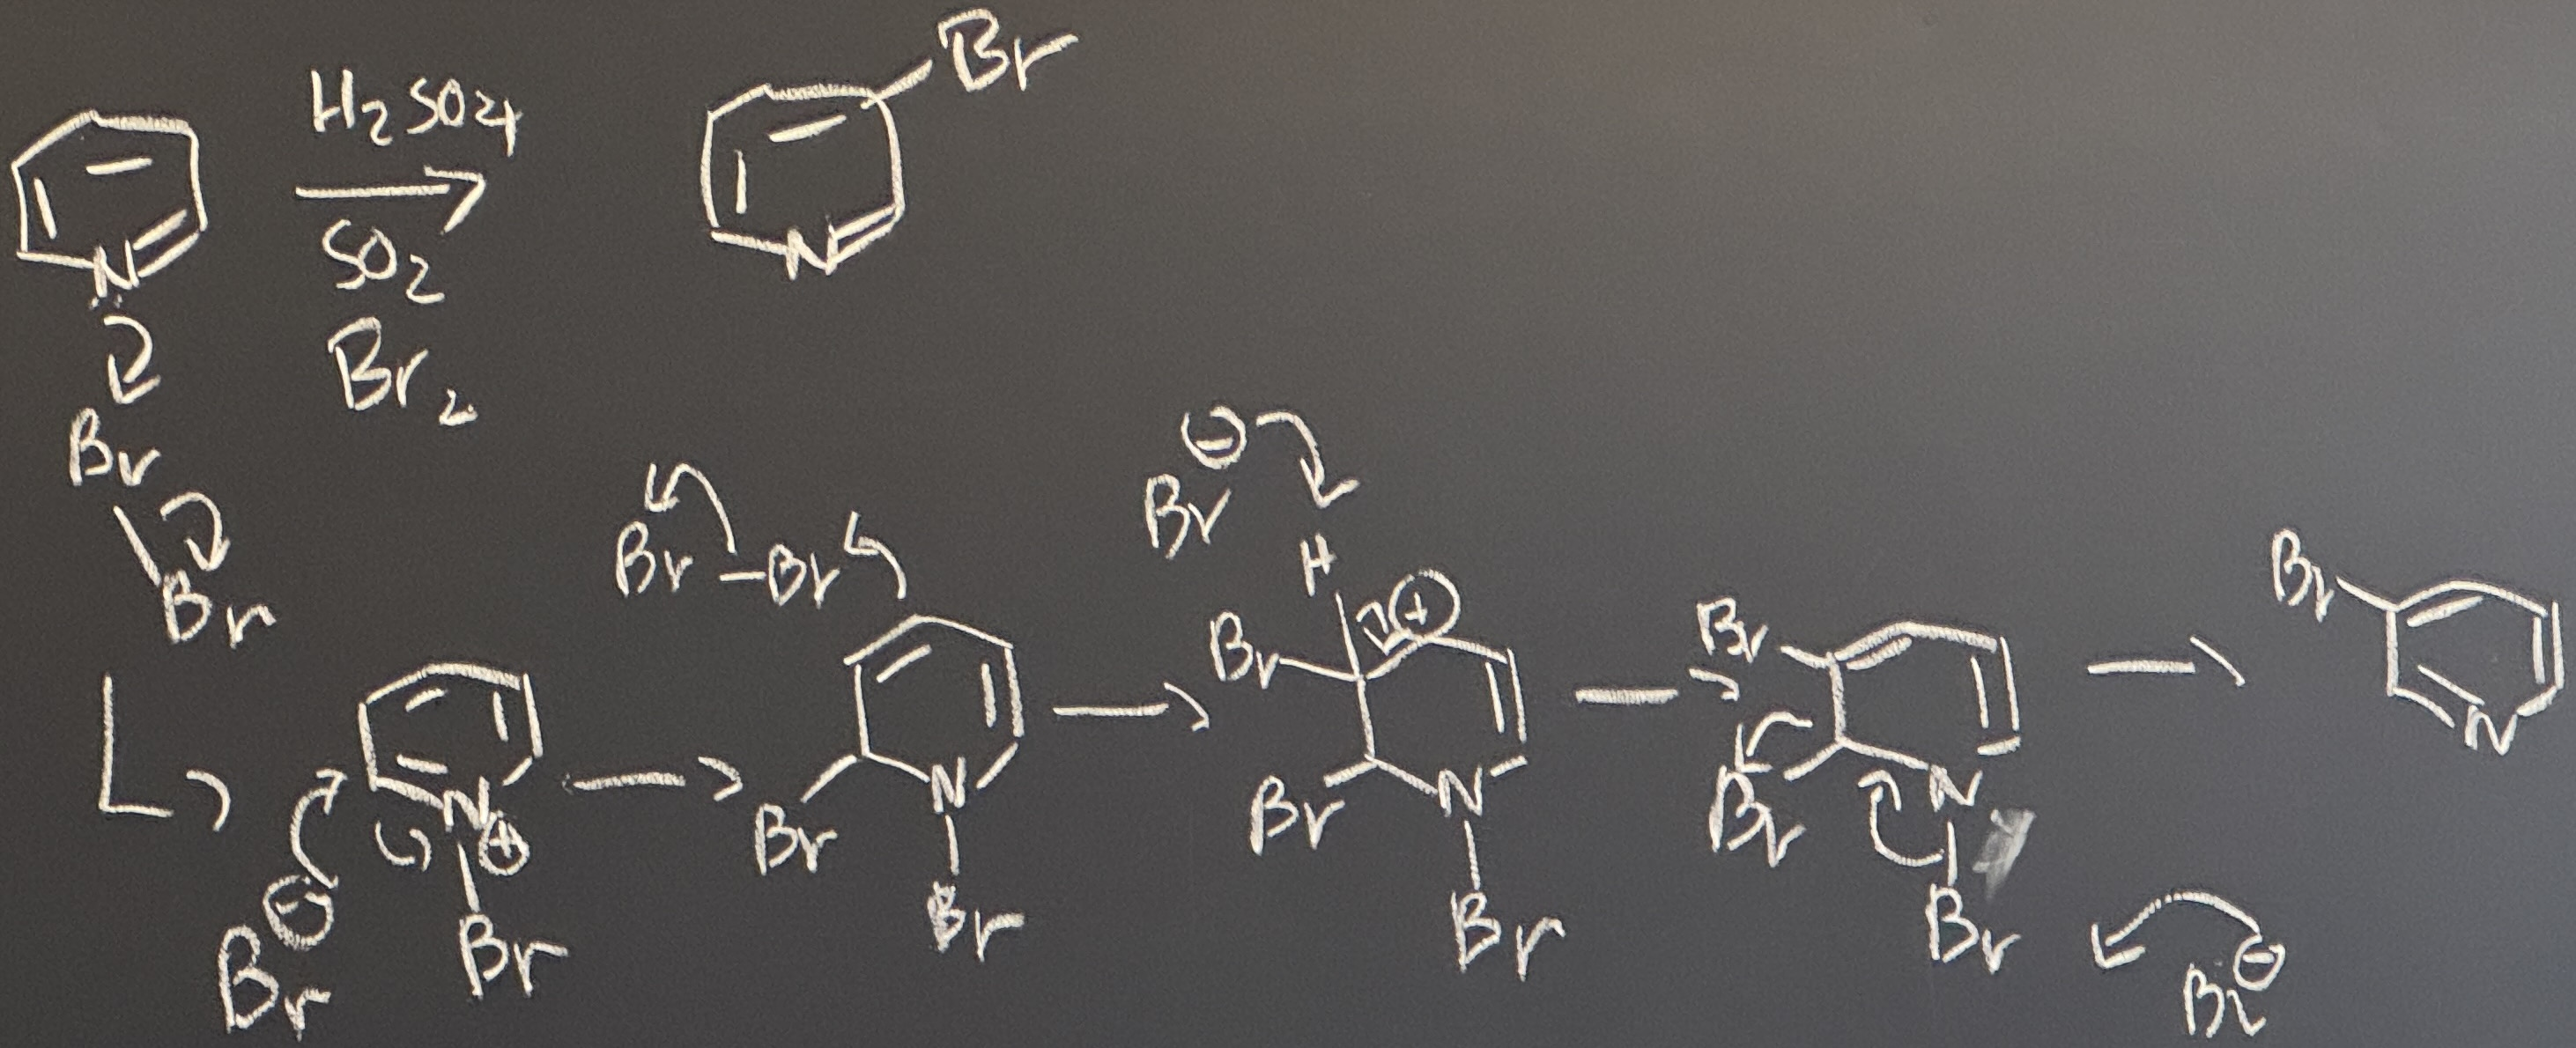
\includegraphics[width=0.6\linewidth]{TTQPy3Br.JPG}
        \caption{TTQ: Pyridine \emph{meta}-bromination.}
        \label{fig:TTQPy3Br}
    \end{figure}
    \begin{itemize}
        \item Uses bromination mechanism from class (see Figure \ref{fig:QI3bromoMech}).
        \item Oleum could be \ce{SO2} or \ce{SO3}.
        \item \ce{Br-} can remove either bromine in the last step.
        \item This gets full credit; it is great, but for the second bromination, it may make more sense to put the bromine on the other side of the compound; the 1,2-dibromide is unfavorable.
        \begin{itemize}
            \item Principle: Large halides on contiguous carbons is just very challenging.
        \end{itemize}
        \item Unclear what the \ce{SO2} does.
        \item Electrophilic reaction $\to$ nucleophilic reaction with dearomatization.
    \end{itemize}
\end{itemize}




\end{document}